\section{Specific Requirements}
\subsection{External interface requirements}
\subsubsection{User interfaces}
There are two user interfaces in our system: one for the smartphone used to access the service; one for the onboard infotainment system of the Car.

%
%
%SMARTPHONE UI
%
%
\begin{figure}[h!]
    \centering
    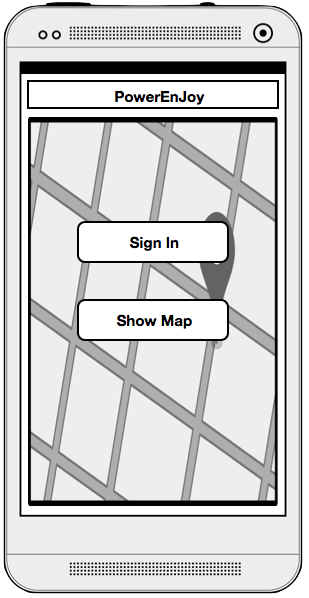
\includegraphics[scale=0.4]{{Figures/Mockup/1FirstScreen.png}}
    \label{fig:1FirstScreen}
    \\From the first screen a user can either sign in, and if necessary create a new account, or consult the map of available Cars.
\end{figure}

\begin{figure}[p!]
    \centering
    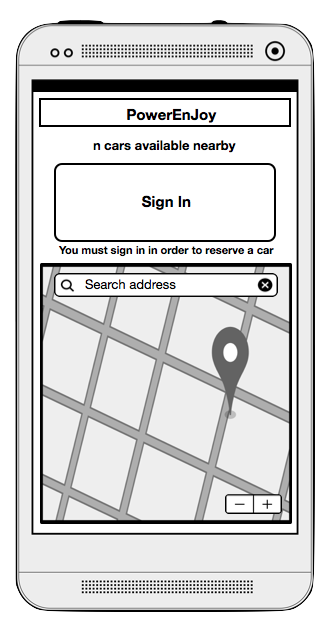
\includegraphics[scale=0.4]{{Figures/Mockup/2MapNotLogged.png}}
    \label{fig:2MapNotLogged}
    \\If a user chooses the map, he will see a map with the position and the remaining battery charge of all the available Cars; he is asked to sign in in order to proceed with the reservation.
\end{figure}


\begin{figure}[p!]
    \centering
    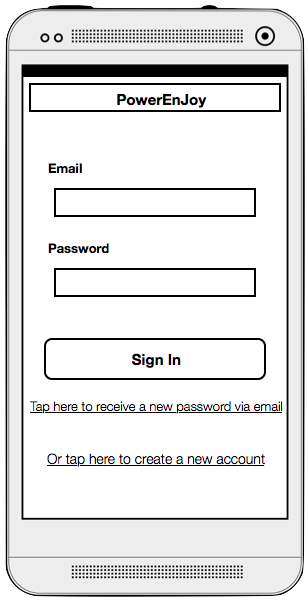
\includegraphics[scale=0.4]{{Figures/Mockup/3LoginForm.png}}
    \label{fig:3LoginForm}
    \\Whether a user started from the map or from the first screen, he will have to either enter his credential or register. In case of forgotten credential he is given the possibility to ask for a new password too.
\end{figure}

\begin{figure}[p!]
    \centering
    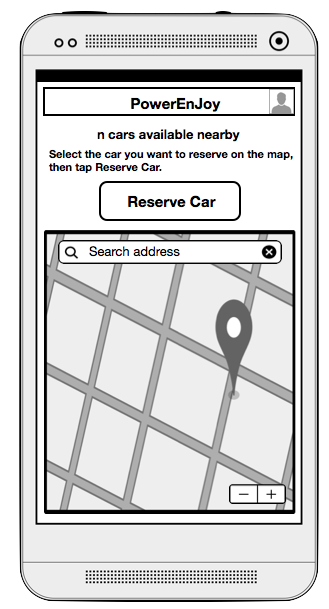
\includegraphics[scale=0.4]{{Figures/Mockup/4CarReservationA}}
    \label{fig:4CarReservationA}
    \\A PowerUser can look for a suitable Car nearby his position, or entering an address in the appropriate bar above the map. After finding a Car the PowerUser can reserve it.
\end{figure}

\begin{figure}[p!]
    \centering
    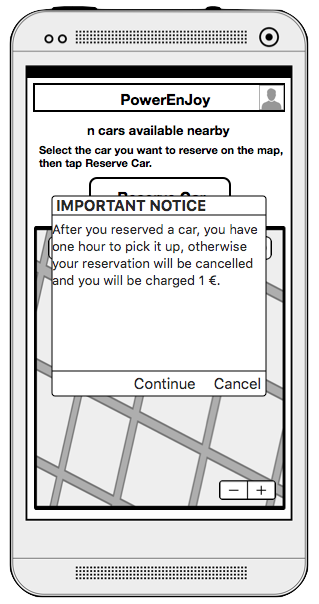
\includegraphics[scale=0.4]{{Figures/Mockup/4CarReservationB.png}}
    \label{fig:4CarReservationB}
    \\Before actually reserving a Car, the system reminds the PowerUser about the one hour expiration of his reservation and the relative penalty fee.
\end{figure}

\begin{figure}[p!]
    \centering
    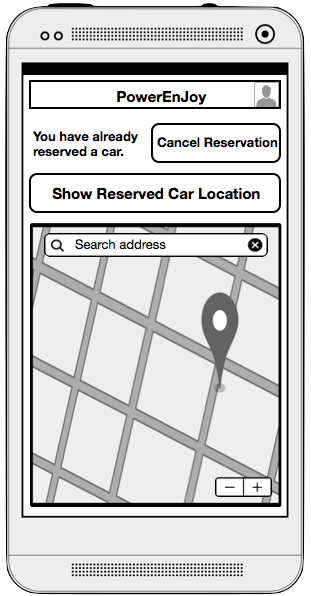
\includegraphics[scale=0.4]{{Figures/Mockup/5CarReserved.png}}
    \label{fig:5CarReserved}
    \\After the selected Car has been reserved, a PowerUser can cancel his reservation or look for his Car thanks to the provided map.
\end{figure}

\begin{figure}[p!]
    \centering
    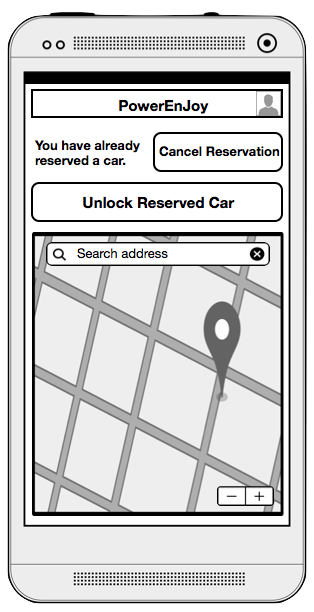
\includegraphics[scale=0.4]{{Figures/Mockup/6CarNearby.png}}
    \label{fig:6CarNearby}
    \\When a PowerUser is near his reserved Car, he is given the possibility to ask the system to unlock it. If the PowerUser changes his mind he can still cancel the reservation, this possibility will remain valid until the PowerUser ignites the engine. 
\end{figure}

\begin{figure}[p!]
    \centering
    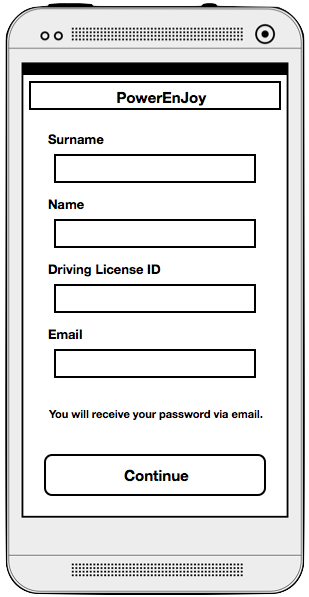
\includegraphics[scale=0.4]{{Figures/Mockup/7RegistrationFormA.png}}
    \label{fig:7RegistrationFormAForm}
    \\This is the first page of the registration procedure; it requires a new user to enter his personal data.
\end{figure}


\begin{figure}[p!]
    \centering
    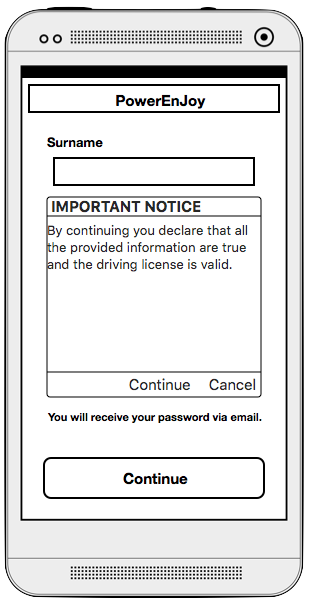
\includegraphics[scale=0.4]{{Figures/Mockup/7RegistrationFormB.png}}
    \label{fig:7RegistrationFormB}
    \\In order to stress the importance of entering real and correct data, the system reminds the user about it.
\end{figure}

\begin{figure}[p!]
    \centering
    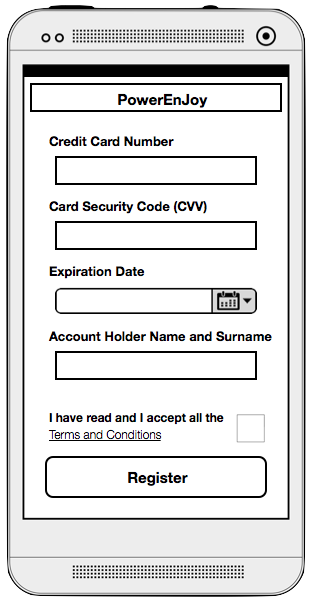
\includegraphics[scale=0.4]{{Figures/Mockup/7RegistrationFormC.png}}
    \label{fig:7RegistrationFormCnForm}
    \\Last page of the registration procedure, the user is asked for his payment information. Furthermore he will have to accept the terms and conditions of the service in order to complete the registration.
\end{figure}

\begin{figure}[p!]
    \centering
    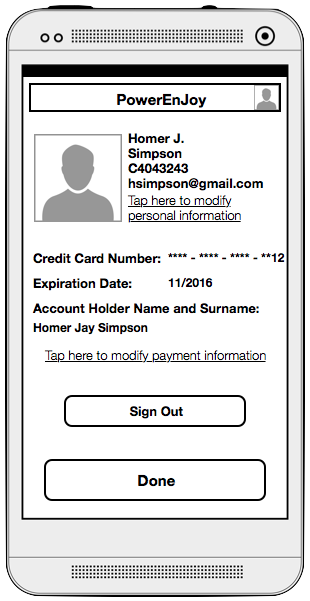
\includegraphics[scale=0.4]{{Figures/Mockup/8PersonalAccountPage.png}}
    \label{fig:8PersonalAccountPage}
    \\A PowerUser can access his personal account page by tapping on the avatar in the up right corner of his smartphone screen. By doing so, this is what he will be shown. From this page it is also possible to modify both personal and payment information.
\end{figure}

\begin{figure}[p!]
    \centering
    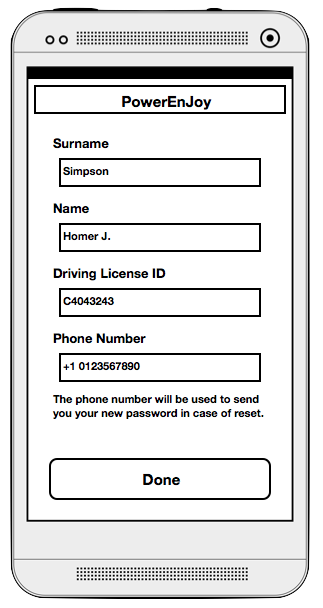
\includegraphics[scale=0.4]{{Figures/Mockup/9PersonalDataModification.png}}
    \label{fig:9PersonalDataModification}
    \\This is the page to be used by a PowerUser in order to modify his personal information.
\end{figure}

\begin{figure}[p!]
    \centering
    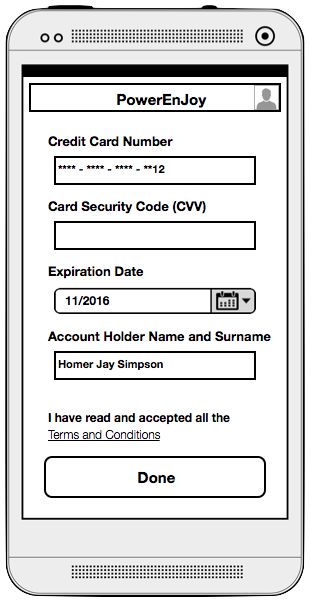
\includegraphics[scale=0.4]{{Figures/Mockup/10PaymentSystemDataModification.png}}
    \label{fig:10PaymentSystemDataModificationForm}
    \\This is the page to be used by a PowerUser in order to modify his payment information.
\end{figure}

%
%
%CAR UI
%
%
\begin{figure}[p!]
    \centering
    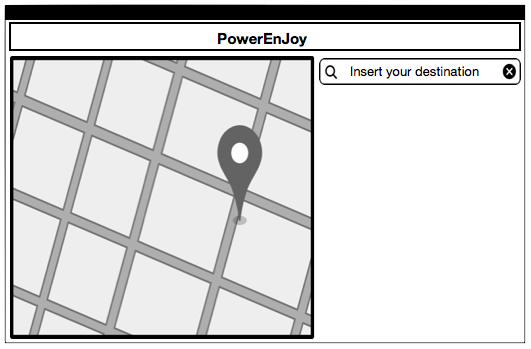
\includegraphics[scale=0.6]{{Figures/Mockup/11FirstCarScreen.png}}
    \label{fig:11FirstCarScreen}
    \\This is the first screen a PowerUser will see when entering in a Car. The map on the left is a placeholder for the third party navigation system.
\end{figure}

\begin{figure}[p!]
    \centering
    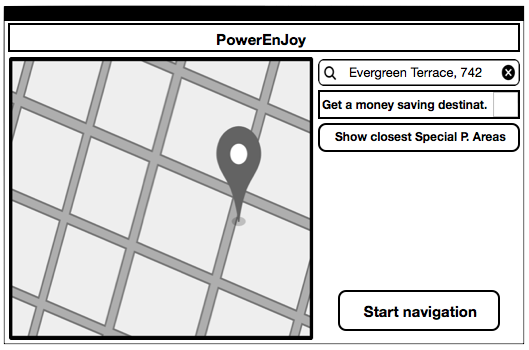
\includegraphics[scale=0.6]{{Figures/Mockup/12aCorrectDestination.png}}
    \label{fig:12aCorrectDestination}
    \\A PowerUser searches for his destination and if it is inside the set of Safe Parking Areas he is allowed to start the navigation system.
\end{figure}

\begin{figure}[p!]
    \centering
    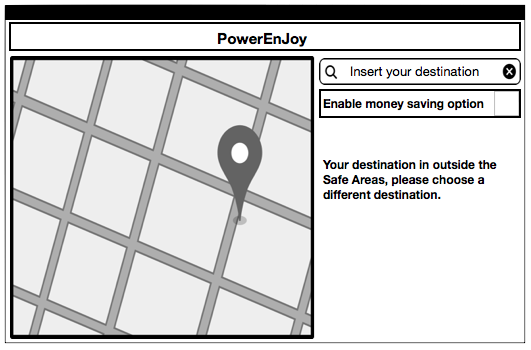
\includegraphics[scale=0.6]{{Figures/Mockup/12bWrongDestination.png}}
    \label{fig:12bWrongDestination}
    \\A PowerUser search for his destination and if it is not inside the set of Safe Parking Areas he is asked to look for another destination.
\end{figure}

\begin{figure}[p!]
    \centering
    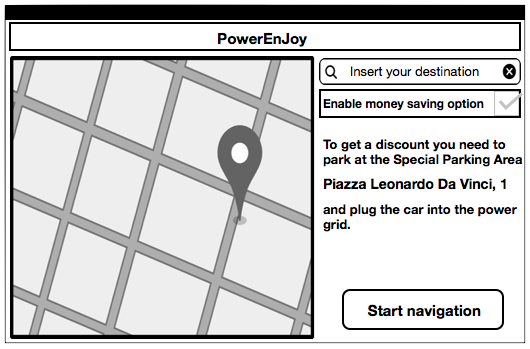
\includegraphics[scale=0.6]{{Figures/Mockup/12cMoneySavingOption.png}}
    \label{fig:12cMoneySavingOption}
    \\When a PowerUser enables the money saving option he is provided with the address of the Special Parking Area where he is supposed to park and plug the car into the power grid.
\end{figure}

\begin{figure}[p!]
    \centering
    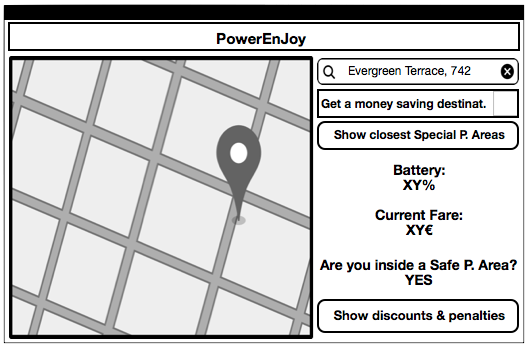
\includegraphics[scale=0.6]{{Figures/Mockup/13Ride.png}}
    \label{fig:13Ride}
    \\This is the screen the PowerUser sees while he is driving. If he needs to change the destination he is free to do that, or if he wants to know more about discounts and penalties he can tap the apposite button.
\end{figure}

\begin{figure}[p!]
    \centering
    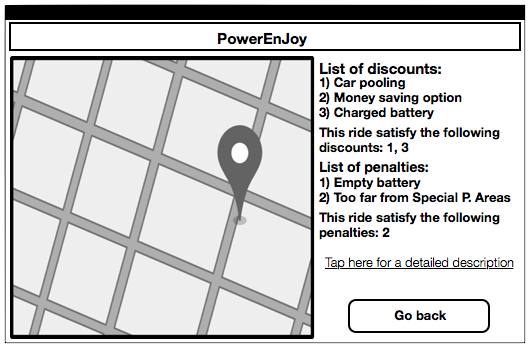
\includegraphics[scale=0.6]{{Figures/Mockup/14DIscountsAndPenalties.png}}
    \label{fig:14DIscountsAndPenalties}
    \\This is the screen that sums up all discounts and penalties, and it also declares explicitly which one is valid at the moment. If a PowerUser needs a more detailed description he just have to tap to show a windows containing all the details and the explanation of each discount and penalty.  
\end{figure}

\newpage

\subsubsection{Hardware interfaces}
The system interfaces directly with sensors and actuators of the Cars, like GPS, door locking and unlocking mechanism, battery sensor, power socket detector.

\subsubsection{Communication interfaces}
The system requires internet connectivity across all involved devices.

\subsubsection{Software interfaces}
The system relies on a third party payment service to issue payment requests, and a third party navigation system for the onboard Car equipment which provides driving directions.

\subsection{Functional requirements}

\newcounter{goalctr}
    \stepcounter{goalctr}
    \subsubsection{Goal \arabic{goalctr}}
    {[}G\arabic{goalctr}{]}
    Allow any kind of user to view the map of the available nearby Cars
    \begin{itemize}
        \item Requirements
        \begin{enumerate}[label={[}R\arabic*{]},series=REQ]
    		    \item Users must have access to a map indicating the user current location.
        		\item Users must be able to pan and scroll a map in any direction.
    		    \item Every available Car must be shown on a map.
    	    	\item Users shall have an input for inserting an address in which center the map.
                \item Users shall have an input to center the map view on their position.
        \end{enumerate}
        \item Domain properties
        \begin{enumerate}[label={[}P\arabic*{]},series=PRO]
                \item B\% and C\% are remaining battery power percentages defined during setup.
    			\item No Car with less than B\% battery charge is taken into account as available for booking.
    			\item No Car that is currently under charging and has less than C\% battery charge is taken into account as available for booking.
        \end{enumerate}
    \end{itemize}
    
    \stepcounter{goalctr}
    \subsubsection{Goal \arabic{goalctr}}
    {[}G\arabic{goalctr}{]}
    Allow Visitor user to register to the service.
    \begin{itemize}
        \item Requirements
        \begin{enumerate}[REQ]
    		    \item Let a Visitor user start the registration wizard while he's still not logged in.
			    \item The registration form must contain input fields for user identity, email, contact info, driving license number and expiration, privacy agreement confirmation, customer notifications and subscriptions options, credit card number and expiration, billing identity.
			    \item The chosen email address must not be already used by another PowerUser.
			    \item The credit card must be verified not to be blocked or expired upon registration.
			    \item The user must receive a system generated password to the registered email address.
        \end{enumerate}
        \item Domain properties
        \begin{enumerate}[PRO]
    			\item None
        \end{enumerate}
    \end{itemize}

    \stepcounter{goalctr}
    \subsubsection{Goal \arabic{goalctr}}
    {[}G\arabic{goalctr}{]}
    Allow Visitor user to log-in and out as a PowerUser.
    \begin{itemize}
        \item Requirements
        \begin{enumerate}[REQ]
			    \item A Visitor user must always see an input to access log-in form as long as he's still not logged in.
		        \item An input to perform log-out must always be available to the PowerUser if he's currently logged in.
        \end{enumerate}
        \item Domain properties
        \begin{enumerate}[PRO]
    			\item None
        \end{enumerate}
    \end{itemize}

    \stepcounter{goalctr}
    \subsubsection{Goal \arabic{goalctr}}
    {[}G\arabic{goalctr}{]}
    Allow PowerUser to check the status of the Car.
    \begin{itemize}
        \item Requirements
        \begin{enumerate}[REQ]
    		    \item For each available Car the PowerUser must be able to view its remaining battery charge.
			    \item For each available Car the PowerUser must be able to view its current position.
        \end{enumerate}
        \item Domain properties
        \begin{enumerate}[PRO]
    			\item None
        \end{enumerate}
    \end{itemize}

    \stepcounter{goalctr}
    \subsubsection{Goal \arabic{goalctr}}
    {[}G\arabic{goalctr}{]}
    Allow PowerUser to reserve a Car.
    \begin{itemize}
        \item Requirements
        \begin{enumerate}[REQ]
    		    \item The PowerUser must have the ability to start the reservation wizard for all and only available Cars.
			    \item The PowerUser must see a reminder about unfulfilled reservation penalty before confirmation.
			    \item Show an input to allow the PowerUser to confirm and finalize the reservation.
			    \item The system shall prevent the PowerUser to reserve more than a Car from the same geographical region at a time.
        \end{enumerate}
        \item Domain properties
        \begin{enumerate}[PRO]
    			\item Each geographical region has its own set of assigned Cars.
        \end{enumerate}
    \end{itemize}
    
    \stepcounter{goalctr}
    \subsubsection{Goal \arabic{goalctr}}
    {[}G\arabic{goalctr}{]}
    Allow PowerUser to cancel a reservation.
    \begin{itemize}
        \item Requirements
        \begin{enumerate}[REQ]
    			\item If a reservation exists for the PowerUser, show him an input to request cancellation.
    			\item The system shall prompt the PowerUser for cancellation confirmation.
    			\item A reservation must be automatically cancelled by the system after 1 hour from its creation.
    			\item If a reservation is cancelled because of timeout, notify the PowerUser about that occurrence.
        \end{enumerate}
        \item Domain properties
        \begin{enumerate}[PRO]
    			\item None
        \end{enumerate}
    \end{itemize}

    \stepcounter{goalctr}
    \subsubsection{Goal \arabic{goalctr}}
    {[}G\arabic{goalctr}{]}
	Allow PowerUser to check the position of the reserved car.
    \begin{itemize}
        \item Requirements
        \begin{enumerate}[REQ]
    	        \item As long as a reservation exists for the PowerUser he must always be able to get the position of the reserved Car on the map.
        \end{enumerate}
        \item Domain properties
        \begin{enumerate}[PRO]
    		    \item None
        \end{enumerate}
    \end{itemize}

    \stepcounter{goalctr}
    \subsubsection{Goal \arabic{goalctr}}
    {[}G\arabic{goalctr}{]}
	Allow PowerUser to unlock and enter the Car when inside the specific range.
    \begin{itemize}
        \item Requirements
        \begin{enumerate}[REQ]
    	        \item The system must be able to remotely unlock the Car.
			    \item The system must be able to compute the distance between the user location and his reserved Car.
			    \item The PowerUser must have an input allowing him to send an unlock request.
			    \item The system must accept the unlock request issued by the PowerUser if and only if the PowerUser is in the unlock allowance area.
			    \item If the unlock request is accepted, the PowerUser must be able to enter the Car.
        \end{enumerate}
        \item Domain properties
        \begin{enumerate}[PRO]
                \item The PowerUser position is always the same as of its mobile device that runs the PowerUser application.
    			\item The PowerUser is considered to be in the unlocking allowance area if the distance to the Car is at most equal to 5 meters.
        \end{enumerate}
    \end{itemize}
    
    \stepcounter{goalctr}
    \subsubsection{Goal \arabic{goalctr}}
    {[}G\arabic{goalctr}{]}
    Allow PowerUser to get driving directions to his destination.
    \begin{itemize}
        \item Requirements
        \begin{enumerate}[REQ]
    			\item The user must be allowed to select a custom destination and start navigating to that location.
        \end{enumerate}
        \item Domain properties
        \begin{enumerate}[PRO]
    			\item Navigation software always provides effective directions to the user if destination it's included in Safe Areas.
        \end{enumerate}
    \end{itemize}
    
    \stepcounter{goalctr}
    \subsubsection{Goal \arabic{goalctr}}
    {[}G\arabic{goalctr}{]}
	Bill the PowerUser for the amount of time spent riding a Car.
    \begin{itemize}
        \item Requirements
        \begin{enumerate}[REQ]
                \item Start counting the billing time from the first engine ignition.
    	        \item Make the system constantly show the updated Total Base Fare on the Car screen.
    	        \item Stop the billing time counter after exactly 1 second after the Car locking.
        \end{enumerate}
        \item Domain properties
        \begin{enumerate}[PRO]
                \item None
        \end{enumerate}
    \end{itemize}

    \stepcounter{goalctr}
    \subsubsection{Goal \arabic{goalctr}}
    {[}G\arabic{goalctr}{]}
    Allow PowerUser to see a list of the closest Special Parking Areas to his destination.
    \begin{itemize}
        \item Requirements
        \begin{enumerate}[REQ]
    		    \item The system must be capable of providing a list of Special Parking Areas sorted by distance from an input location.
			    \item PowerUser must be allowed anytime during the navigation to input a custom location and be acknowledged about all nearest Special Parking Areas from the selected location.
        \end{enumerate}
        \item Domain properties
        \begin{enumerate}[PRO]
    			\item None
        \end{enumerate}
    \end{itemize}
    
    \stepcounter{goalctr}
    \subsubsection{Goal \arabic{goalctr}}
    {[}G\arabic{goalctr}{]}
    Allow PowerUser to keep track of the current charged fare.
    \begin{itemize}
        \item Requirements
        \begin{enumerate}[REQ]
    			\item Show on the Car screen a live updated counter indicating the Total Base Fare amount that the user will actually pay if the ride ends in that same moment, as long as the ride is being charged.
        \end{enumerate}
        \item Domain properties
        \begin{enumerate}[PRO]
    			\item The PowerUser stops being charged in the same moment the Car is locked.
        \end{enumerate}
    \end{itemize}
    
    \stepcounter{goalctr}
    \subsubsection{Goal \arabic{goalctr}}
    {[}G\arabic{goalctr}{]}
    Allow PowerUser to check whether he can be eligible for any discount or penalty.
    \begin{itemize}
        \item Requirements
        \begin{enumerate}[REQ]
    			\item Provide through Car screen an input to access an overview of all discounts and penalties.
    			\item For each shown discount or penalty allow the PowerUser to get a brief informal description of corresponding criteria.
    			\item For each shown discount or penalty allow the PowerUser to know if the current ride satisfies all needed criteria at the moment.
        \end{enumerate}
        \item Domain properties
        \begin{enumerate}[PRO]
    			\item None
        \end{enumerate}
    \end{itemize}
 
    \stepcounter{goalctr}
    \subsubsection{Goal \arabic{goalctr}}
    {[}G\arabic{goalctr}{]}
    Allow PowerUser to get a money saving alternative destination.
    \begin{itemize}
        \item Requirements
        \begin{enumerate}[REQ]
    			\item While a ride destination is selected for navigation, show the PowerUser the option to get a money saving destination proposal.
    			\item Always show to PowerUser an input to get money saving proposal even if there exists a selected destination.
    			\item The destination proposal must correspond to the nearest (w.r.t. PowerUser selected destination) Special Parking Area where there are less than N\# Cars attached to the power source.
    			\item If the PowerUser accepts the money saving destination proposal, the current selected destination must be updated accordingly.
        \end{enumerate}
        \item Domain properties
        \begin{enumerate}[PRO]
                \item N\# is an integer number defined during setup.
    			\item Special Parking Areas provide at least N\# power sockets as exclusively available to PowerEnJoy customers.
        \end{enumerate}
    \end{itemize}
 
    \stepcounter{goalctr}
    \subsubsection{Goal \arabic{goalctr}}
    {[}G\arabic{goalctr}{]}
    Allow the system to lock the Car in a Safe Parking Area at the end of the ride.
    \begin{itemize}
        \item Requirements
        \begin{enumerate}[REQ]
    			\item The system must lock the Car if its position belong to the set of Safe Parking Areas, engine is stopped, all doors are closed and S\# seconds passed from the last door closure.
        \end{enumerate}
        \item Domain properties
        \begin{enumerate}[PRO]
                \item S\# is a time-span defined during setup.
    			\item At least a free parking slot is available for the user among all Safe Parking Areas.
        \end{enumerate}
    \end{itemize} 
 
    \stepcounter{goalctr}
    \subsubsection{Goal \arabic{goalctr}}
    {[}G\arabic{goalctr}{]}
    Allow the system to apply penalty or discount according to the given criteria.
    \begin{itemize}
        \item Requirements
        \begin{enumerate}[REQ]
    			\item The system shall apply a discount of 10\% on the last ride Total Base Fare if the number of passengers at the end of the ride is greater or equal to the number of passengers at the start of the ride and the number of passengers at the start of the ride was at least 3, driver included.
    			\item The system shall apply a discount of 20\% on the last ride Total Base Fare if the remaining battery power at the end of the ride is greater or equal then 50\%.
    			\item The system shall apply a discount of 30\% on the last ride Total Base Fare if the Car position at the end of the ride is within a Special Parking Areas and the power socket is detected as connected two minutes from the Car locking.
    			\item The system shall apply a penalty of 30\% on the last ride Total Base Fare if the position of the Car at the time of locking is more than 3km far from the nearest power grid station or the remaining battery power is less than 20\% and the Car is not detected as attached to power grid within two minutes from locking.
        \end{enumerate}
        \item Domain properties
        \begin{enumerate}[PRO]
    	        \item None
    	\end{enumerate}
    \end{itemize} 

    \stepcounter{goalctr}
    \subsubsection{Goal \arabic{goalctr}}
    {[}G\arabic{goalctr}{]}
    Let the system bill the PowerUser for the total ride fare and issue a payment request for that amount at the end of the ride.
    \begin{itemize}
        \item Requirements
        \begin{enumerate}[REQ]
    			\item The system must charge the PowerUser the total fare after two minutes and an half from the Car locking.
    			\item The system must issue the payment request to the payment processor provider.	
    			\item The system must bill the PowerUser a penalty of 1$\euro$ as soon as a reservation he made expires ny timeout.
    			\item The PowerUser shall be notified of any money charge by email.
    			\item The PowerUser shall be notified of the payment transaction result.
        \end{enumerate}
        \item Domain properties
        \begin{enumerate}[PRO]
    			\item None
        \end{enumerate}
    \end{itemize}


\subsection{Use cases}


\subsubsection{Cars Map Exploration}
\begin{tabular}{| l | p{8cm} |}
\hline
\textbf{Actor}      &       Visitor \\
\hline
\textbf{Goal}       &       [G1]\\
\hline
\textbf{Entry Condition} &  NULL\\
\hline
\textbf{Event Flow}     &   1.	a.\\&
                                            2.	b.\\&
                                            3.	c.\\&
                                            4.  d.\\
\hline
\textbf{Output Condition} & conditionExplanation\\
\hline
\textbf{Exceptions} &       •   ex1.\\& 
                            •	ex2.\\&
                            •	ex3.\\& 
                           How expections are managed.\\
\hline
\end{tabular} 

\subsubsection{Service Registration}
\begin{tabular}{| l | p{8cm} |}
\hline
\textbf{Actor}      &       Visitor \\
\hline
\textbf{Goal}       &       [G2]\\
\hline
\textbf{Entry Condition} &  NULL\\
\hline
\textbf{Event Flow}     &   1.	a.\\&
                                            2.	b.\\&
                                            3.	c.\\&
                                            4.  d.\\
\hline
\textbf{Output Condition} & conditionExplanation\\
\hline
\textbf{Exceptions} &       •   ex1.\\& 
                            •	ex2.\\&
                            •	ex3.\\& 
                           How expections are managed.\\
\hline
\end{tabular} 


\subsubsection{Sign In}
\begin{tabular}{| l | p{8cm} |}
\hline
\textbf{Actor}      &       Visitor \\
\hline
\textbf{Goal}       &       [G3]\\
\hline
\textbf{Entry Condition} &  NULL\\
\hline
\textbf{Event Flow}     &   1.	a.\\&
                                            2.	b.\\&
                                            3.	c.\\&
                                            4.  d.\\
\hline
\textbf{Output Condition} & conditionExplanation\\
\hline
\textbf{Exceptions} &       •   ex1.\\& 
                            •	ex2.\\&
                            •	ex3.\\& 
                           How expections are managed.\\
\hline
\end{tabular} 


\subsubsection{Sign Out}
\begin{tabular}{| l | p{8cm} |}
\hline
\textbf{Actor}      &       PowerUser \\
\hline
\textbf{Goal}       &       [G3]\\
\hline
\textbf{Entry Condition} &  Existent PowerUser session.\\
\hline
\textbf{Event Flow}     &   1.	a.\\&
                                            2.	b.\\&
                                            3.	c.\\&
                                            4.  d.\\
\hline
\textbf{Output Condition} & conditionExplanation\\
\hline
\textbf{Exceptions} &       •   ex1.\\& 
                            •	ex2.\\&
                            •	ex3.\\& 
                           How expections are managed.\\
\hline
\end{tabular} 


\subsubsection{Car Status Checking}
\begin{tabular}{| l | p{8cm} |}
\hline
\textbf{Actor}      &       PowerUser \\
\hline
\textbf{Goal}       &       [G4]\\
\hline
\textbf{Entry Condition} &  NULL\\
\hline
\textbf{Event Flow}     &   1.	a.\\&
                                            2.	b.\\&
                                            3.	c.\\&
                                            4.  d.\\
\hline
\textbf{Output Condition} & conditionExplanation\\
\hline
\textbf{Exceptions} &       •   ex1.\\& 
                            •	ex2.\\&
                            •	ex3.\\& 
                           How expections are managed.\\
\hline
\end{tabular} 

\subsubsection{Car Reservation}
\begin{tabular}{| l | p{8cm} |}
\hline
\textbf{Actor}      &       PowerUser \\
\hline
\textbf{Goal}       &       [G5]\\
\hline
\textbf{Entry Condition} &  NULL\\
\hline
\textbf{Event Flow}     &   1.	a.\\&
                                            2.	b.\\&
                                            3.	c.\\&
                                            4.  d.\\
\hline
\textbf{Output Condition} & conditionExplanation\\
\hline
\textbf{Exceptions} &       •   ex1.\\& 
                            •	ex2.\\&
                            •	ex3.\\& 
                           How expections are managed.\\
\hline
\end{tabular} 


\subsubsection{Reservation Cancellation}
\begin{tabular}{| l | p{8cm} |}
\hline
\textbf{Actor}      &       PowerUser \\
\hline
\textbf{Goal}       &       [G6]\\
\hline
\textbf{Entry Condition} &  NULL\\
\hline
\textbf{Event Flow}     &   1.	a.\\&
                                            2.	b.\\&
                                            3.	c.\\&
                                            4.  d.\\
\hline
\textbf{Output Condition} & conditionExplanation\\
\hline
\textbf{Exceptions} &       •   ex1.\\& 
                            •	ex2.\\&
                            •	ex3.\\& 
                           How expections are managed.\\
\hline
\end{tabular} 


\subsubsection{Reserved Car Information}
\begin{tabular}{| l | p{8cm} |}
\hline
\textbf{Actor}      &       PowerUser \\
\hline
\textbf{Goal}       &       [G7]\\
\hline
\textbf{Entry Condition} &  NULL\\
\hline
\textbf{Event Flow}     &   1.	a.\\&
                                            2.	b.\\&
                                            3.	c.\\&
                                            4.  d.\\
\hline
\textbf{Output Condition} & conditionExplanation\\
\hline
\textbf{Exceptions} &       •   ex1.\\& 
                            •	ex2.\\&
                            •	ex3.\\& 
                           How expections are managed.\\
\hline
\end{tabular} 


\subsubsection{Reserved Car Unlocking}
\begin{tabular}{| l | p{8cm} |}
\hline
\textbf{Actor}      &       PowerUser \\
\hline
\textbf{Goal}       &       [G8]\\
\hline
\textbf{Entry Condition} &  NULL\\
\hline
\textbf{Event Flow}     &   1.	a.\\&
                                            2.	b.\\&
                                            3.	c.\\&
                                            4.  d.\\
\hline
\textbf{Output Condition} & conditionExplanation\\
\hline
\textbf{Exceptions} &       •   ex1.\\& 
                            •	ex2.\\&
                            •	ex3.\\& 
                           How expections are managed.\\
\hline
\end{tabular} 


\subsubsection{Getting Driving Directions}
\begin{tabular}{| l | p{8cm} |}
\hline
\textbf{Actor}      &       PowerUser \\
\hline
\textbf{Goal}       &       [G9]\\
\hline
\textbf{Entry Condition} &  NULL\\
\hline
\textbf{Event Flow}     &   1.	a.\\&
                                            2.	b.\\&
                                            3.	c.\\&
                                            4.  d.\\
\hline
\textbf{Output Condition} & conditionExplanation\\
\hline
\textbf{Exceptions} &       •   ex1.\\& 
                            •	ex2.\\&
                            •	ex3.\\& 
                           How expections are managed.\\
\hline
\end{tabular} 


\subsubsection{???}
\begin{tabular}{| l | p{8cm} |}
\hline
\textbf{Actor}      &       SBL \\
\hline
\textbf{Goal}       &       [G10]\\
\hline
\textbf{Entry Condition} &  NULL\\
\hline
\textbf{Event Flow}     &   1.	a.\\&
                                            2.	b.\\&
                                            3.	c.\\&
                                            4.  d.\\
\hline
\textbf{Output Condition} & conditionExplanation\\
\hline
\textbf{Exceptions} &       •   ex1.\\& 
                            •	ex2.\\&
                            •	ex3.\\& 
                           How expections are managed.\\
\hline
\end{tabular} 


\subsubsection{Special Parking Areas Listing}
\begin{tabular}{| l | p{8cm} |}
\hline
\textbf{Actor}      &       PowerUser \\
\hline
\textbf{Goal}       &       [G11]\\
\hline
\textbf{Entry Condition} &  NULL\\
\hline
\textbf{Event Flow}     &   1.	a.\\&
                                            2.	b.\\&
                                            3.	c.\\&
                                            4.  d.\\
\hline
\textbf{Output Condition} & conditionExplanation\\
\hline
\textbf{Exceptions} &       •   ex1.\\& 
                            •	ex2.\\&
                            •	ex3.\\& 
                           How expections are managed.\\
\hline
\end{tabular} 


\subsubsection{Current Charged Fare Viewing}
\begin{tabular}{| l | p{8cm} |}
\hline
\textbf{Actor}      &       PowerUser \\
\hline
\textbf{Goal}       &       [G12]\\
\hline
\textbf{Entry Condition} &  NULL\\
\hline
\textbf{Event Flow}     &   1.	a.\\&
                                            2.	b.\\&
                                            3.	c.\\&
                                            4.  d.\\
\hline
\textbf{Output Condition} & conditionExplanation\\
\hline
\textbf{Exceptions} &       •   ex1.\\& 
                            •	ex2.\\&
                            •	ex3.\\& 
                           How expections are managed.\\
\hline
\end{tabular} 


\subsubsection{Discounts And Penalties ???(checking)}
\begin{tabular}{| l | p{8cm} |}
\hline
\textbf{Actor}      &       PowerUser \\
\hline
\textbf{Goal}       &       [G13]\\
\hline
\textbf{Entry Condition} &  NULL\\
\hline
\textbf{Event Flow}     &   1.	a.\\&
                                            2.	b.\\&
                                            3.	c.\\&
                                            4.  d.\\
\hline
\textbf{Output Condition} & conditionExplanation\\
\hline
\textbf{Exceptions} &       •   ex1.\\& 
                            •	ex2.\\&
                            •	ex3.\\& 
                           How expections are managed.\\
\hline
\end{tabular} 


\subsubsection{Money Saving Suggestion}
\begin{tabular}{| l | p{8cm} |}
\hline
\textbf{Actor}      &       PowerUser \\
\hline
\textbf{Goal}       &       [G14]\\
\hline
\textbf{Entry Condition} &  NULL\\
\hline
\textbf{Event Flow}     &   1.	a.\\&
                                            2.	b.\\&
                                            3.	c.\\&
                                            4.  d.\\
\hline
\textbf{Output Condition} & conditionExplanation\\
\hline
\textbf{Exceptions} &       •   ex1.\\& 
                            •	ex2.\\&
                            •	ex3.\\& 
                           How expections are managed.\\
\hline
\end{tabular} 


\subsubsection{Car Locking}
\begin{tabular}{| l | p{8cm} |}
\hline
\textbf{Actor}      &       SBL \\
\hline
\textbf{Goal}       &       [G15]\\
\hline
\textbf{Entry Condition} &  NULL\\
\hline
\textbf{Event Flow}     &   1.	a.\\&
                                            2.	b.\\&
                                            3.	c.\\&
                                            4.  d.\\
\hline
\textbf{Output Condition} & conditionExplanation\\
\hline
\textbf{Exceptions} &       •   ex1.\\& 
                            •	ex2.\\&
                            •	ex3.\\& 
                           How expections are managed.\\
\hline
\end{tabular} 


\subsubsection{Discounts And Penalties ???(application)}
\begin{tabular}{| l | p{8cm} |}
\hline
\textbf{Actor}      &       SBL \\
\hline
\textbf{Goal}       &       [G16]\\
\hline
\textbf{Entry Condition} &  NULL\\
\hline
\textbf{Event Flow}     &   1.	a.\\&
                                            2.	b.\\&
                                            3.	c.\\&
                                            4.  d.\\
\hline
\textbf{Output Condition} & conditionExplanation\\
\hline
\textbf{Exceptions} &       •   ex1.\\& 
                            •	ex2.\\&
                            •	ex3.\\& 
                           How expections are managed.\\
\hline
\end{tabular} 


\subsubsection{Payment Deduction}
\begin{tabular}{| l | p{8cm} |}
\hline
\textbf{Actor}      &       SBL \\
\hline
\textbf{Goal}       &       [G17]\\
\hline
\textbf{Entry Condition} &  NULL\\
\hline
\textbf{Event Flow}     &   1.	a.\\&
                                            2.	b.\\&
                                            3.	c.\\&
                                            4.  d.\\
\hline
\textbf{Output Condition} & conditionExplanation\\
\hline
\textbf{Exceptions} &       •   ex1.\\& 
                            •	ex2.\\&
                            •	ex3.\\& 
                           How expections are managed.\\
\hline
\end{tabular} 